\section{Data Transfer}

\begin{concept}{Data Transfer Overview}\\
ARM Cortex-M uses a load/store architecture:
\begin{itemize}
  \item Memory can only be accessed through load and store instructions
  \item All other operations work on registers
  \item Data processing only between registers
  \item Various addressing modes for flexible memory access:
    \begin{itemize}
      \item Immediate offset: Fixed displacement from base
      \item Register offset: Variable displacement using register
      \item Pre-indexed: Address calculated before access
      \item Post-indexed: Address calculated after access
    \end{itemize}
    \item Steps: Load operands $\rightarrow$ Execute $\rightarrow$ Store result
\end{itemize}
\end{concept}

\begin{remark}
Two main approaches to memory access, the other one:

\textbf{Register Memory Architecture (e.g., Intel x86)}:
    \begin{itemize}
      \item Operations can use memory operands directly
      \item Results can be written directly to memory
      \item More flexible but more complex instructions
    \end{itemize}
\end{remark}

\begin{formula}{Load Instructions}\\
Main load instructions for moving data into registers:
\begin{itemize}
  \item \textbf{MOVS} (Move and Set flags):
    \begin{itemize}
      \item Register to Register: \texttt{MOVS R1, R2}
      \item 8-bit immediate: \texttt{MOVS R1, \#0x1C}
      \item Constant: \texttt{MOVS R1, \#MyConst}
      \item Limitations: Only 8-bit immediates, only low registers
    \end{itemize}
  \item \textbf{LDR} (Load Register):
    \begin{itemize}
      \item 32-bit literal: \texttt{LDR R1, \#0xA1B2C3D4}
      \item PC-relative: \texttt{LDR R1, [PC, \#12]}
      \item Pseudo instruction: \texttt{LDR R1, =MyConst}
      \item Register indirect: \texttt{LDR R1, [R2]}
      \item Immediate offset: \texttt{LDR R1, [R2, \#4]}
      \item Register offset: \texttt{LDR R1, [R2, R3]}
    \end{itemize}
  \item \textbf{LDRB} (Load Register Byte):
    \begin{itemize}
      \item Loads 8-bit value
      \item Bits 31 to 8 are set to zero (Zero extension to 32 bits)
      \item Common for arrays of bytes
    \end{itemize}
  \item \textbf{LDRH} (Load Register Half-word):
    \begin{itemize}
      \item Loads 16-bit value
      \item Bits 31 to 16 are set to zero (Zero extension to 32 bits)
      \item Common for arrays of half-words
    \end{itemize}
  \item \textbf{LDRSB/LDRSH} (Load Signed Register Byte/Half-word):
    \begin{itemize}
      \item Sign extension to 32 bits
      \item Used for signed small integers
    \end{itemize}
\end{itemize}
\end{formula}



\begin{example2}{Load Instruction Examples}
\begin{lstlisting}[language=armasm, style=basesmol]
; MOV examples
MOVS    R1, #0xFF       ; Load immediate 255
MOVS    R2, R1          ; Copy R1 to R2
; LDR examples
LDR     R1, =0x12345678 ; Load 32-bit constant
LDR     R2, [R1]        ; Load from address in R1
LDR     R3, [R1, #4]    ; Load with offset
LDR     R4, [R1, R2]    ; Load with register offset
; Byte/Half-word loads
LDRB    R1, [R2]        ; Load unsigned byte
LDRSB   R1, [R2]        ; Load signed byte
LDRH    R1, [R2]        ; Load unsigned half-word
LDRSH   R1, [R2]        ; Load signed half-word
\end{lstlisting}
\end{example2}

\begin{formula}{Store Instructions}\\
Instructions for storing data from registers to memory:
\begin{itemize}
  \item \textbf{STR} (Store Register):
    \begin{itemize}
      \item Basic store: \texttt{STR R1, [R2]}
      \item With immediate offset: \texttt{STR R1, [R2, \#0x04]}
      \item With register offset: \texttt{STR R1, [R2, R3]}
      \item Word-aligned addresses only
    \end{itemize}
  \item \textbf{STRB} (Store Register Byte):
    \begin{itemize}
      \item Stores lowest 8 bits of register
      \item No alignment requirements
    \end{itemize}
  \item \textbf{STRH} (Store Register Half-word):
    \begin{itemize}
      \item Stores lowest 16 bits of register
      \item Must be half-word aligned
    \end{itemize}
\end{itemize}
\end{formula}

\subsubsection{Memory Access}

\begin{corollary}{Memory Layout}
for array elements and instructions:

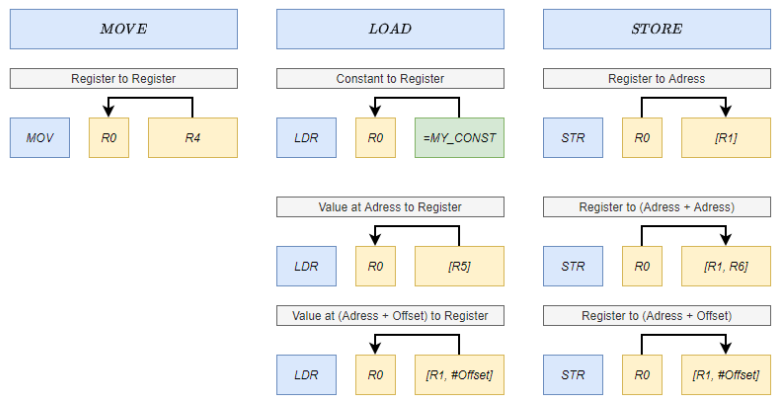
\includegraphics[width=\linewidth]{images/memory_layout.png}
\end{corollary}

\begin{remark}
Size considerations:
\begin{itemize}
  \item Array elements: 3 * 4 Bytes
  \item Instructions: 5 * 2 Bytes
  \item Literals (0x08): 1 * 4 Bytes
\end{itemize}
\end{remark}

\begin{KR}{Memory Access Patterns} in Load/Store Architecture \\
Steps for accessing memory:
\begin{enumerate}
  \item Determine required data size (byte, half-word, word)
  \item Choose appropriate load/store instruction
  \item Calculate correct memory address
  \item Consider alignment requirements
  \item Load/store data using proper addressing mode
\end{enumerate}
\end{KR}

\begin{concept}{Memory Alignment}
Important alignment rules:
\begin{itemize}
  \item \textbf{Word access (LDR/STR)}:
    \begin{itemize}
      \item Address must be multiple of 4
      \item Misaligned access causes fault
    \end{itemize}
  \item \textbf{Half-word access (LDRH/STRH)}:
    \begin{itemize}
      \item Address must be multiple of 2
    \end{itemize}
  \item \textbf{Byte access (LDRB/STRB)}:
    \begin{itemize}
      \item No alignment requirements
    \end{itemize}
  \item \textbf{Stack operations}:
    \begin{itemize}
      \item SP must be word-aligned
      \item PUSH/POP automatically maintain alignment
    \end{itemize}
\end{itemize}
\end{concept}

\begin{example2}{Basic Data Transfer Operations}
Common data transfer operations:
\begin{lstlisting}[language=armasm, style=basesmol]
;Load operations
MOVS R1, #42      ;Load immediate value
MOVS R2, R1       ;Copy register
LDR  R3, =0x1234  ;Load 32-bit constant
LDR  R4, [R3]     ;Load from memory
LDRB R5, [R3, #1] ;Load byte with offset

;Store operations
STR  R1, [R2]     ;Store word
STRB R1, [R2, #4] ;Store byte with offset
STRH R1, [R2, R3] ;Store half-word with register offset
\end{lstlisting}
\end{example2}


\begin{KR}{Common Data Transfer Patterns}\\
1. Copy memory block:
\begin{lstlisting}[language=armasm, style=basesmol]
    ; R0 = source, R1 = dest, R2 = count
loop
    LDR     R3, [R0], #4    ; Load and increment
    STR     R3, [R1], #4    ; Store and increment
    SUBS    R2, #1          ; Decrement counter
    BNE     loop           ; Continue if not zero
\end{lstlisting}

2. Initialize memory block:
\begin{lstlisting}[language=armasm, style=basesmol]
    ; R0 = start, R1 = value, R2 = count
loop
    STR     R1, [R0], #4    ; Store and increment
    SUBS    R2, #1          ; Decrement counter
    BNE     loop           ; Continue if not zero
\end{lstlisting}

3. Search memory:
\begin{lstlisting}[language=armasm, style=basesmol]
    ; R0 = start, R1 = value to find, R2 = count
loop
    LDR     R3, [R0], #4    ; Load and increment
    CMP     R3, R1          ; Compare with value
    BEQ     found           ; Branch if found
    SUBS    R2, #1          ; Decrement counter
    BNE     loop           ; Continue if not zero
not_found
    ; Handle not found case
found
    ; Handle found case
\end{lstlisting}
\end{KR}

\begin{concept}{Register Access}\\
For operations involving high registers (R8-R15):
\begin{itemize}
  \item Use MOV for register transfers (works with all registers but only for reg/reg transfers)
  \item Cannot use MOVS with high registers
\end{itemize}
\end{concept}

\columnbreak

\subsubsection{Arrays}

\begin{concept}{Memory Access}
Loading and storing array elements:

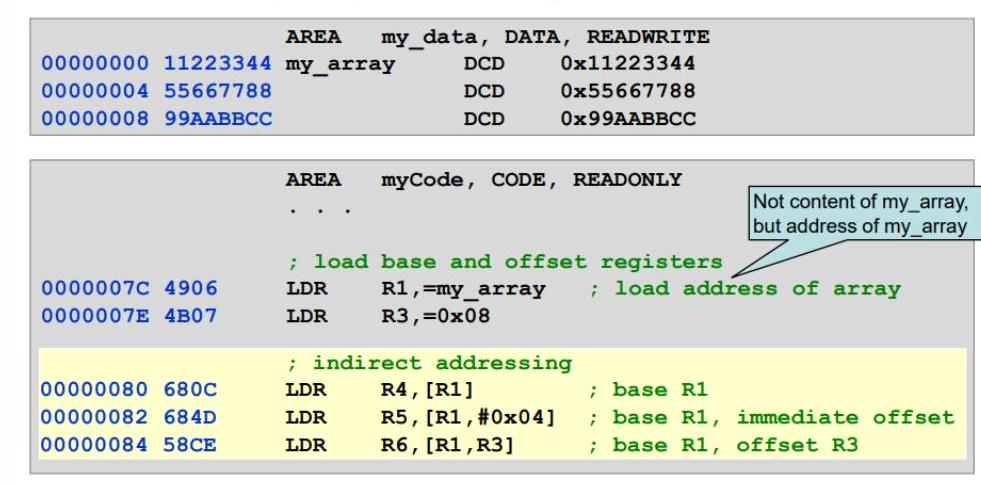
\includegraphics[width=\linewidth]{images/2024_12_29_79e6b22f503fb7b4f718g-03(1)}

\begin{itemize}
  \item my\_array = 3 * 4 Bytes
  \item Instructions = 5 * 2 Bytes
  \item Literals (0x08) = 1 * 4 Bytes
\end{itemize}
\end{concept}

\begin{code}{Accessing Array Elements}\\
Steps for array access:

1. Calculate element offset:
   \begin{itemize}
     \item Byte array: offset = index
     \item Half-word array: offset = index * 2
     \item Word array: offset = index * 4
   \end{itemize}

2. Choose appropriate instruction:
   \begin{itemize}
     \item LDRB/STRB for byte arrays
     \item LDRH/STRH for half-word arrays
     \item LDR/STR for word arrays
   \end{itemize}

Example implementation:
\begin{lstlisting}[language=armasm, style=basesmol]
; Access array[i] where i is in R1
; Array base address in R0

; For byte array
LDRB    R2, [R0, R1]    ; R2 = array[i]

; For half-word array
LSLS    R2, R1, #1      ; R2 = i * 2
LDRH    R3, [R0, R2]    ; R3 = array[i]

; For word array
LSLS    R2, R1, #2      ; R2 = i * 4
LDR     R3, [R0, R2]    ; R3 = array[i]
\end{lstlisting}
\end{code}


\columnbreak


\subsubsection{Multiple Register Transfer}

\begin{definition}{Multiple Register Transfer}\\
LDM (Load Multiple) and STM (Store Multiple):
\begin{itemize}
  \item Load/store multiple registers in one instruction
  \item More efficient than individual loads/stores
  \item Used for stack operations (PUSH/POP)
  \item Register list specified in curly braces
\end{itemize}

Example:
\begin{lstlisting}[language=armasm, style=basesmol]
LDM     R0!, {R1-R4}    ; Load 4 consecutive words
STM     R0!, {R1-R4}    ; Store 4 consecutive words
\end{lstlisting}
\end{definition}

\begin{example2}{Multiple Data Transfer}
Loading/Storing multiple registers:
\begin{lstlisting}[language=armasm, style=basesmol]
; Store multiple registers
PUSH    {R0-R3, LR}     ; Push registers to stack

; Load multiple registers
POP     {R0-R3, PC}     ; Pop and return

; Load multiple memory locations
LDM     R0!, {R1-R4}    ; Load 4 words, update R0

; Store multiple memory locations
STM     R0!, {R1-R4}    ; Store 4 words, update R0
\end{lstlisting}
\end{example2}

\begin{KR}{Multi-Word Data Transfer}\\
For transferring data larger than 32 bits:

1. Loading 96-bit value:
\begin{lstlisting}[language=armasm, style=basesmol]
    ; Load 96-bit value from memory
    ; R3(MSW), R2, R1(LSW) contain result
    ; Memory address in R6
    LDM     R6, {R1-R3}     ; Load all words at once
    
    ; Alternative using individual loads:
    LDR     R1, [R6]        ; Load LSW
    LDR     R2, [R6, #4]    ; Load middle word
    LDR     R3, [R6, #8]    ; Load MSW
\end{lstlisting}

2. Storing 96-bit value:
\begin{lstlisting}[language=armasm, style=basesmol]
    ; Store 96-bit value to memory
    ; R3(MSW), R2, R1(LSW) contain data
    ; Memory address in R6
    STM     R6, {R1-R3}     ; Store all words at once
    
    ; Alternative using individual stores:
    STR     R1, [R6]        ; Store LSW
    STR     R2, [R6, #4]    ; Store middle word
    STR     R3, [R6, #8]    ; Store MSW
\end{lstlisting}
\end{KR}

\subsubsection{Stack Operations}

\begin{concept}{Stack Access Instructions}\\
Special variants of LDM/STM for stack operations:
\begin{itemize}
  \item \textbf{PUSH \{register list\}}:
    \begin{itemize}
      \item Decrements SP
      \item Stores registers
      \item Example: \texttt{PUSH \{R0-R3, LR\}}
    \end{itemize}
  \item \textbf{POP \{register list\}}:
    \begin{itemize}
      \item Loads registers
      \item Increments SP
      \item Example: \texttt{POP \{R0-R3, PC\}}
    \end{itemize}
\end{itemize}
\end{concept}

\begin{remark}
Important considerations:
\begin{itemize}
  \item Always check alignment requirements
  \item Be aware of endianness (STM32 is little-endian)
  \item Consider using multiple register transfer for efficiency
  \item Manage literal pool placement in code
  \item Stack operations must maintain SP word alignment
\end{itemize}
\end{remark}

\subsubsection{Pseudo Instructions}

\begin{definition}{LDR Pseudo Instructions}\\
The LDR pseudo instruction \texttt{LDR Rx, =value} is expanded by the assembler:

1. For literal values:
\begin{itemize}
  \item Assembler creates 'literal pool' at convenient location
  \item Allocates and initializes memory with DCD directive
  \item Uses PC-relative addressing to access value
\end{itemize}

2. For addresses:
\begin{itemize}
  \item Places address in literal pool
  \item Generates PC-relative load instruction
\end{itemize}

Example:
\begin{lstlisting}[language=armasm, style=basesmol]
    LDR     R1, =0xFF55AAB0  ; Pseudo instruction
    ; Assembler converts to:
    LDR     R1, [PC, #offset]
    ...
    DCD     0xFF55AAB0      ; In literal pool
\end{lstlisting}
\end{definition}

\begin{example2}{Pseudo Instruction vs Direct Load}
The difference between LDR forms:
\begin{lstlisting}[language=armasm, style=basesmol]
    LDR     R5, mylita      ; Loads value at mylita
    LDR     R5, =mylita     ; Loads address of mylita

mylita  DCD     0xFF001122   ; Data definition
\end{lstlisting}

First instruction loads 0xFF001122, second loads address of mylita.
\end{example2}

\begin{concept}{Pseudo-Instructions}\\
A pseudo-instruction like \texttt{LDR Rn, =literal}:
\begin{itemize}
  \item Does not directly translate to machine code
  \item Is expanded by assembler into actual instructions
  \item Decomposed into:
    \begin{itemize}
      \item DCD directive for place reservation
      \item LDR instruction to load from that position
    \end{itemize}
  \item Can handle:
    \begin{itemize}
      \item Address literals (position in memory)
      \item Constant literals (known at assembly time)
    \end{itemize}
\end{itemize}
\end{concept}